%%%%%%%%%%%%%%%%%%%%%%%%%%%%%%%%%%%%%%%%%%%%%%%%%%%%%%%%%%%%%%%%%%%%%%%%
% 
% LaTeX Template
%
%%%%%%%%%%%%%%%%%%%%%%%%%%%%%%%%%%%%%%%%%%%%%%%%%%%%%%%%%%%%%%%%%%%%%%%%

%------------------------------------------------------------------------------------------------
%	DOCUMENT CONFIGURATIONS
%------------------------------------------------------------------------------------------------

% DOCUMENT
%   - Properties
\documentclass[a4paper,11pt]{report} % Sets a two-sided A4 sized paper.
                                         % (Two-sided for LaTeX to distinguish between odd/even
                                         % pages while using headers and footers.)
\linespread{1.15}                         % Default space between lines
                                    % Margin sizes defined in headers_and_footers file.
\usepackage[nottoc,numbib]{tocbibind}    % Makes References section appear in the Table of contents (nottoc). Conuts the References like section.
\usepackage{lastpage}                    % To get the total number of pages.

%   - Sectioning
\usepackage{titlesec}                   % Extra features for sectioning
    % The following lines create: \subsubsubsection{}
    
    
%%%%%%%%% From here: creation of \subsubsubsection{} %%%%%%%%%
    \titleclass{\subsubsubsection}{straight}[\subsection]

    \newcounter{subsubsubsection}[subsubsection]
    \renewcommand\thesubsubsubsection{\thesubsubsection.\arabic{subsubsubsection}}
    \renewcommand\theparagraph{\thesubsubsubsection.\arabic{paragraph}} % optional; useful if paragraphs are to be numbered

    \titleformat{\subsubsubsection}
      {\normalfont\normalsize\bfseries}{\thesubsubsubsection}{1em}{}
    \titlespacing*{\subsubsubsection}
    {0pt}{3.25ex plus 1ex minus .2ex}{1.5ex plus .2ex}

    \makeatletter
    \renewcommand\paragraph{\@startsection{paragraph}{5}{\z@}%
      {3.25ex \@plus1ex \@minus.2ex}%
      {-1em}%
      {\normalfont\normalsize\bfseries}}
    \renewcommand\subparagraph{\@startsection{subparagraph}{6}{\parindent}%
      {3.25ex \@plus1ex \@minus .2ex}%
      {-1em}%
      {\normalfont\normalsize\bfseries}}
    \def\toclevel@subsubsubsection{4}
    \def\toclevel@paragraph{5}
    \def\toclevel@paragraph{6}
    \def\l@subsubsubsection{\@dottedtocline{4}{7em}{4em}}
    \def\l@paragraph{\@dottedtocline{5}{10em}{5em}}
    \def\l@subparagraph{\@dottedtocline{6}{14em}{6em}}
    \makeatother

    \setcounter{secnumdepth}{4}
    \setcounter{tocdepth}{4}
%%%%%%%%% Until here: creation of \subsubsubsection{} %%%%%%%%%


%\let\oldsection\section % This line and the following force sections to start on odd pages.
%\def\section{\cleardoublepage\oldsection}

\newcommand*{\blankpage}{%
    \vspace*{\fill}
        \begin{center}
            (This page was intentionally left in blank.)
        \end{center}
    \vspace{\fill}
}
\makeatletter
\renewcommand*{\cleardoublepage}{\clearpage\if@twoside \ifodd\c@page\else
\blankpage
\thispagestyle{empty}
\newpage
\if@twocolumn\hbox{}\newpage\fi\fi\fi}
\makeatother

% WRITING
%   - Math/Chemistry/...
\usepackage{amsmath}                % Mathematical features.
    % Section numbering
    \numberwithin{equation}{section}    % Equation numbering by section
    \numberwithin{table}{section}       % Table numbering by section
    \numberwithin{figure}{section}      % Table numbering by section
\usepackage{amssymb}                % Symbols.
\usepackage[version=3]{mhchem}                 % Chemical equation typesetting. i.e.: \ce{CO2 + C <=> 2CO}
\usepackage{siunitx}                % Simplifies the usage of values with units.
                                    % i.e.: "\SI{5.4}{kg·m^{-1}·s^{-2}}"
                                    % instead of "5.4 kg·m$ ^{-1} $·s$ ^{-2} $"
\usepackage{eurosym}                % Use EURO symbol (\euro)

%%   - Language
\usepackage[utf8]{inputenc}         % Required for the usage of characters like 'ñ', 'ú', ...
%\renewcommand{\figurename}{Figura}  % In captions, print "Figura" (in Catalan) instead of
                                    % "Figure" (English default name).
%\renewcommand{\tablename}{Tabla}
%\renewcommand{\contentsname}{Índice}
%\renewcommand{\refname}{Bibliografía}

%   - Text
%\let\oldsection\section             % This line and the nextone force sections to start always in new odd pages.
%\def\section{\cleardoublepage\oldsection} %
\usepackage[none]{hyphenat}         % [none] Prevents any hyphenation throughout the document.
                                    % (hyphenation -> "separació per síl·labes")
\sloppy                             % Forces wrapping at word boundaries by relaxing the interword space constraints.
%\usepackage{indentfirst}            % Forces indentation from paragraphs after a section.
                                    % (see notes 1 and 2)
\setlength\parindent{1cm}           % Removes all indentation from paragraphs.
%\newenvironment{paragraphs}{\setlength\parindent{1cm}}{\setlength\parindent{0cm}}
                                    % "\begin{paragraphs}" will create an environment where
                                    % indentation from paragraphs is activated.
\usepackage[font=footnotesize]{caption} % Captions
\setlength{\abovecaptionskip}{0pt}      %
\setlength{\belowcaptionskip}{0pt}      %
\usepackage{lmodern}                % Allow the use of font size larger tha 25pt
\usepackage[T1]{fontenc}            %

% GRAPHICS, TABLES AND OTHERS
\usepackage{graphicx}               % Required for the inclusion of images.
\usepackage{float}                  % Required for some float properties.
\usepackage{pdfpages}               % Required for the inclusion of PDF files.
\usepackage{multirow,longtable,array,booktabs,tabularx} % More features for tables.
\usepackage{enumerate}              % Gives the enumerate environment an optional argument which
                                    % determines the style in which the counter is printed.
\usepackage{enumitem}               % Extra options for "enumerate" lists
\usepackage{color}                  % Use some color options.
\usepackage{colortbl}               % Use some other color options.
	\definecolor{UPC_blue}{RGB}{67,142,197}
	\definecolor{lightgrey}{RGB}{166,166,166}
\usepackage{hyperref}               % Provides LeTeX the hability to create hyperlinks.

\usepackage{inputenc}         % It makes possible to use roman numbers for the pages before the first chapter and arabic for the rest of the document

\usepackage{booktabs}
\usepackage{xcolor,colortbl}
\usepackage{pstricks}
\usepackage{blindtext}
\usepackage{transparent}
\usepackage{etoolbox}
\usepackage{pdflscape}
\usepackage{amsmath}
\usepackage{amsfonts}
\usepackage{amssymb}
\usepackage{graphicx}
\usepackage{eurosym}
\usepackage{wrapfig}
\usepackage{mathdots}
\usepackage{caption}
\usepackage{cite}
\usepackage{mathrsfs}
\usepackage{float}
\usepackage{import}
\usepackage{makecell}
\usepackage{booktabs}
\usepackage{caption}
\usepackage{subcaption}
\usepackage{textcomp}

%   - NOTES
% (1) LaTeX implements a style that doesn't indent the first paragraph after a section heading. There are coherent reasons for this. Some typography rules state that first indent should be suppressed only after a centered title and that all other paragraphs must be indented.
% (2) We have already removed all indentation from paragraphs with the command "\setlength\parindent{0cm}", but when using the environment we've created "escrit" we set indent to 1cm. Then, if this environment is used right after a section the first indent will be suppressed unless we use the package "indentfirst". % Document Configurations

%-----------------------------------------------------------------------------
%	REPORT INFORMATION
%-----------------------------------------------------------------------------

%%% MAIN INFORMATION %%%

% School
\newcommand{\School}{ESEIAAT}
\newcommand{\researcherDept}{Airports design and construction}
% Degree
\newcommand{\Degree}{Master's degree in Aerospace Engineering}

% Department
\newcommand{\Department}{Airports design and construction}

% Secció (Secció de Terrassa)
\newcommand{\Seccio}{Secció de Terrassa}

% Course
\newcommand{\Course}{220304 - Airports design and construction}

% Students (if you don't use that much students, leave them in blank)
\newcommand{\Studi}	{Fontanes Molina, Pol}

% Customer:
\newcommand{\Director}{Montanyà Puig, Joan}
\newcommand{\CoDirector}{Williams, Earle}

% Project Name
\newcommand{\ProjectName}{BEKASI-EAST JAKARTA AIRPORT}

% Acronym
\newcommand{\Acronym}{AIR SIDE}

% Short Name
\newcommand{\ShortName}{Director Plan}

% Kind of document
\newcommand{\DocType}{Report}

% Page number preceding (leave in blank if nothing is required)
% Suggestion: R, RA, B, D, T referred to report, report attachments, budget, drawings or technical sheets
\newcommand{\precPage}{R}


% Date of the document (Delivery date)
	% Day
	\newcommand{\DocDateD}{10}
	% Month
	\newcommand{\DocDateM}{12}
	% Year
	\newcommand{\DocDateY}{2017}

%-----------------------------------------------------------------------------
% Don't touch this unless you know what you are doing!

% Generation of Group Code
\newcommand{\GrCode}{{\GrNum} EA-\GrTerm\GrYr} 

% Generation of the date format
\newcommand{\DocDate}{\DocDateD-\DocDateM-\DocDateY}  % Document information

%-----------------------------------------------------------------------------
%	HEADERS AND FOOTERS
%-----------------------------------------------------------------------------

% Changes default margins.
\usepackage[left=3cm,right=3cm,top=2.5cm,bottom=2.5cm]{geometry}
   \setlength{\headheight}{50pt}         % Header Space.
   \setlength{\textheight}{640pt}        % Text height.
   \setlength{\footskip}{30pt}           % Foot Space.

\usepackage{fancyhdr}
	\pagestyle{fancy} % Headers and footers -> "fancy" style.
	
	% Obtain the name of the section:
	\renewcommand{\sectionmark}[1]{\markright{Section \thesection : #1}}
	\renewcommand{\chaptermark}[1]{\markleft{Chapter \thechapter : #1}} 

	\fancyhf{} % Clear all headers and footers fields

% Package info and examples
%		% O/E = Odd/Even page // L/C/R = Left/Center/Right field
%	\fancyhead[LE]{\hspace{-10pt}
%		\raisebox{-\height+12pt}{
%		
\includegraphics[height=30pt]{./doc_config/images/UPC_dpt}
%		}
%	}
%	\fancyhead[RE]{\bf \Department}
%	\fancyhead[LO]{\bf \DocType}
%	\fancyhead[RO]{\bf \emph{\ProjectName}}
%	\fancyfoot[LE,RO]{\thepage} % Adds customized pages numbers



%-----------------------------------------------
% General headers and footers of the document:
%-----------------------------------------------
	% Headers
	\fancyhead[LO]{\textbf{\rightmark}} % Section mark
	\fancyhead[RO]{
\includegraphics[height=25pt]{./doc_config/images/logo}}
	\fancyhead[LE]{\textbf{\rightmark}}
	\fancyhead[RE]{
\includegraphics[height=25pt]{./doc_config/images/logo}}

	% Footers
	\fancyfoot[CE,CO]{\precPage{} - \thepage}
	\fancyfoot[LO,RE]{\textbf{\Acronym}}

	\renewcommand{\headrulewidth}{0.5pt} % Header decorative line
	\renewcommand{\footrulewidth}{0.5pt} % Footer decorative line
	\renewcommand{\chaptermark}[1]{%
\markboth{#1}{}}
\renewcommand{\sectionmark}[1]{\markright{#1}}


%-----------------------------------------------
% Headers and footers for pages where chapter starts:
%-----------------------------------------------
\fancypagestyle{plain}{
	%Headers
	\fancyhead[LO]{\textbf{\leftmark}} % Section mark
	\fancyhead[RO]{
\includegraphics[height=25pt]{./doc_config/images/logo}}
	\fancyhead[LE]{\textbf{\leftmark}}
	\fancyhead[RE]{
\includegraphics[height=25pt]{./doc_config/images/logo}}
	%Footers
	\fancyfoot[CE]{\precPage{} - \thepage}
	\fancyfoot[CO]{\precPage{} - \thepage}
	\fancyfoot[LO,RE]{\textbf{\Acronym}}
	
	\renewcommand{\headrulewidth}{0.5pt} % Header decorative line
	\renewcommand{\footrulewidth}{0.5pt} % Footer decorative line
}


%-----------------------------------------------
% Cover headers and footers:
%-----------------------------------------------

	\fancypagestyle{CoverPage}{ % This creates a new headers and footers page style.
	                            % To use it type "\thispagestyle{FirstPage}" on the first page.
	                                % (right after "\maketitle")
		\fancyhf{}
		%\fancyfoot[C]{Group \GrCode \hfill [\DocDate]}
		\renewcommand{\headrulewidth}{0pt}
		\renewcommand{\footrulewidth}{0pt}
	}


%-----------------------------------------------
% No headers nor footers page (ie: Back cover)
%-----------------------------------------------

	\fancypagestyle{EmptyPage}{
		\fancyhf{}
		\renewcommand{\headrulewidth}{0pt}
		\renewcommand{\footrulewidth}{0pt}
	} % Headers and footers

%-----------------------------------------------------------------------------
%	USER DEFINED ENVIRONMENTS
%-----------------------------------------------------------------------------

% Itemize with reduced vertyical space between items
\newenvironment{itemize_rvs}
{ \begin{itemize}
    \setlength{\itemsep}{0pt}
    \setlength{\parskip}{0pt}
    \setlength{\parsep}{0pt}     }
{ \end{itemize}                  }

% Standard names

% Titles and sections structures
\newcommand{\subpart}[1]{\mbox{ }\\\noindent\textbf{#1}}
\newcommand{\subsubpart}[1]{\mbox{ }\\\indent\underline{#1}}
\newcommand{\subsubsubpart}[1]{\mbox{ }\\\indent\indent\textit{#1}}

% Figure/table source
\newcommand{\source}[1]{\caption*{\hfill Source: {#1}} } % User defined environments

% Paragraph formatting
\setlength{\parindent}{0pt}

\usepackage{epigraph}
\usepackage{tocloft}
\usepackage{multicol}
\usepackage[T1]{fontenc}
\usepackage{titlesec, blindtext, color}
\usepackage{float}
\usepackage{url}
\definecolor{gray75}{gray}{0.75}
\newcommand{\hsp}{\hspace{20pt}}
\titleformat{\chapter}[hang]{\Huge\bfseries}{\thechapter\hsp\textcolor{gray75}{|}\hsp}{0pt}{\Huge\bfseries}

\renewcommand{\familydefault}{\sfdefault}

\begin{document}

%-----------------------------------------------------------------------------
%	Project Charter Cover
%-----------------------------------------------------------------------------

\thispagestyle{CoverPage}

% Centered cover page

\begin{center}\bf


\includegraphics[width=0.2\textwidth]{./doc_config/images/logo.png}\\
%\large \researcherDept

\vspace{50pt}

%{\large \School}

\vspace{6pt}


\includegraphics[width=0.6\textwidth]{./doc_config/images/UPC_ESEIAAT.jpg}

\vspace{50pt}

%{\Huge \ProjectName}\\
{\fontsize{24pt}{20pt}\selectfont \ProjectName}

\vspace{10pt}

{\fontsize{20pt}{20pt}\selectfont \Acronym}

%\includegraphics[width=0.4\textwidth]{./doc_config/images/DF_logo}

\textcolor{UPC_blue}{\rule{\textwidth}{.6pt}}

{\Large \DocType}

\end{center}

\vspace{50pt}

\textbf{Degree:} \Degree

\textbf{Course:} \Course

\textbf{Delivery date:} \DocDate\\

\vspace{10pt}

%\textbf{Students:} \Studi
\textbf{Students:} Abiétar Moreno, Sergi; Delgado Chicote, Miguel; Fernández Porta, Sergi; Fernández Sanz, Sergio; Fontanes Molina, Pol and Vidal Pedrola, Xavier

%\textbf{Director:} \Director

%\textbf{Co-Director:} \CoDirector % COVER
\newpage\thispagestyle{EmptyPage}
\mbox{}\newpage

\pagenumbering{roman}

% TABLE OF CONTENTS
\setcounter{tocdepth}{3}
\tableofcontents
\pagebreak

%\mbox{}\newpage
\renewcommand{\cfttabnumwidth}{4em}
\listoftables
\pagebreak

%\mbox{}\newpage
\renewcommand{\cftfignumwidth}{4em}
\listoffigures


% DOCUMENT SECTIONS

\newpage
\pagenumbering{arabic}

\newpage
\setlength{\parskip}{1em}
%\input{./sections/AIM}

\chapter{Prognosis}

	\section{Aviation context in Indonesia}
		\subsection{Airport location}
		\subsection{Current traffic}
		\subsection{Ocupation factor}
	
	\section{Reference aircraft}
		\subsection{Aircraft type}
		\subsection{Conclusions}
		
	\section{Forecast computation}
		\subsection{Flights on standard day}
		\subsection{Surface distribution}
\chapter{Terminal building distribution}
	\section{Surface distribution}
	
	The terminal building interiors will be distributed according to the FAA criteria. This method has been chosen because it differentiates between domestic and international passenger flows, which are very well defined at this airport.
	
	\noindent In order to manage and distribute the space available, the forecasted traffic predicted in the prognosis is to be used.
	
	\noindent In first place, as shown in  table  \ref{table:FAAdomestic}, the surface corresponding to domestic traffic is distributed. According to prognosis data, the number of domestic passengers at design hour will be of 4850.
	
	\begin{table}[ht!]
	\label{table:FAAdomestic}
	\centering
	\begin{tabular}{|c|c|c|c|}
	\hline
	\textbf{Surface} & \textbf{\% out of total} & \textbf{m2/pax} & \textbf{m2 total}\\
	\hline
	\textbf{Departures} & 0.0435 & 0.609 & 2953.65 \\
	\hline
	\textbf{Arrivals} & 0.0435 & 0.609 & 2953.65\\
	\hline
	\textbf{Waiting lobby} & 0.0739 & 1.035 & 5019.75\\
	\hline
	\textbf{Restrooms} & 0.013 & 0.183 & 887.55\\
	\hline
	\textbf{Kitchens} & 0.0652 & 0.913 & 4428.05 \\
	\hline
	\textbf{Restaurants} & 0.0652 & 0.913 & 4428.05\\
	\hline
	\textbf{Offices} & 0.1957 & 2.739 & 13284.15\\
	\hline
	\textbf{Other} & 0.0217 & 0.304 & 1474.4\\
	\hline
	\textbf{Circulation} & 0.4783 & 6.696 & 32475.6\\
	\hline
	\textbf{TOTAL} & & & \textbf{67904.85}\\
	\hline
	\end{tabular}
	\caption{Estimated surfaces according to FAA (domestic flights).}
	\end{table}
	
	In second place, as shown in table \ref{table:FAAinternational}, the surface corresponding to international traffic is distributed. According to prognosis data, the number of international passenger at design hour will be of 3168.
	
	
	\begin{table}[ht!]
	\label{table:FAAinternational}
	\centering
	\begin{tabular}{|c|c|c|c|}
	\hline
	\textbf{Surface} & \textbf{\% out of total} & \textbf{m2/pax} & \textbf{m2 total}\\
	\hline
	\textbf{Departures} & 0.0435 & 0.609 & 2953.65 \\
	\hline
	\textbf{Arrivals} & 0.0435 & 0.609 & 2953.65\\
	\hline
	\textbf{Waiting lobby} & 0.0739 & 1.035 & 5019.75\\
	\hline
	\textbf{Restrooms} & 0.013 & 0.183 & 887.55\\
	\hline
	\textbf{Kitchens} & 0.0652 & 0.913 & 4428.05 \\
	\hline
	\textbf{Offices} & 0.1957 & 2.739 & 13284.15\\
	\hline
	\textbf{Other} & 0.0217 & 0.304 & 1474.4\\
	\hline
	\textbf{General circulation} & 0.307 & 6.145 & 19467.36\\
	\hline
	\textbf{Immigration} & 0.042 & 0.838 & 2654.78\\
	\hline
	\textbf{Customs} & 0.084 & 1.676 & 5309.57\\
	\hline
	\textbf{Health} & 0.028 & 0.559 & 1770.91\\
	\hline
	\textbf{Other checkpoints} & 0.006 & 0.112 & 354.816\\
	\hline
	\textbf{Circulation} & 0.198 & 3.966 & 12564.28\\
	\hline
	\textbf{TOTAL} & & & \textbf{63363.17}\\
	\hline
	\end{tabular}
	\caption{Estimated surfaces according to FAA (international  flights).}
	\end{table}
	
	Nevertheless, due to our airport structure and preliminary design, some of these areas are going to be shared between domestic and international passengers. This will allow to tighten the space and reduce the extension of the terminal building, which will be too extense for the number of passengers at design hour.
	
	Therefore, the final dimensioning of the airport will be as follows, shown in table \ref{table:FAAtotal}:
	
	\begin{table}[ht!]\label{table:FAAtotal}
	\centering
	\begin{tabular}{|c|c|c|c|c|c|}
	\hline
	\textbf{General (shared)} & \textbf{m2} & \textbf{Domestic} & \textbf{m2} & \textbf{International} & \textbf{m}2\\
	\hline
	\textbf{Departures} & 4725.56 & \textbf{Waiting lobby} & 5019.75 & \textbf{Immigration} & 2654.78\\
	\hline
	\textbf{Arrivals} & 4724.56 & \textbf{Circulation }& 32475.6 & \textbf{Customs} & 5309.57\\
	\hline
	\textbf{Restaurants} & 7082.83 & & & \textbf{Health} & 1770.91\\
	\hline
	\textbf{Offices} & 21248.50 & & & \textbf{Other checkpoints} & 354.81\\
	\hline
	\textbf{Other} & 2358.27 & & & \textbf{Circulation} & 12562.3\\
	\hline
	\textbf{Restrooms} & 1419.77 & & & \textbf{General circulation} & 19456.36\\
	\hline
	\textbf{Kitchens} & 7082.83 & & & \textbf{Waiting lobby} & 3009.60\\
	\hline
	\textbf{TOTAL} & \textbf{48641.34} & & \textbf{37495.35} & & \textbf{45131.33}\\
	\hline
	\end{tabular}
	\caption{Total surface distribution of terminal building.}
	\end{table}
	
	The total surface of the terminal building area, dedicated to passengers and airport management is of 131267 $\mathrm{m^2}$.
	
	\section{Dimensioning of elements}
\begin{enumerate}
\item \textbf{Check-in counters:} in order to define the check-in area, we have to determine the queueing area and the counters area. Considering the following parameters:
\begin{table}[ht!]
\centering
\begin{tabular}{|c|c|c|}
\hline
PHP(dep) & 2000 & 50\% for arrivals and departures\\
\hline 
b & 0 & Connecting pax not processed in airside\\
\hline
y & 20 min & Average ocuppation time\\
\hline 
s & 1.9 $\mathrm{m^2}$ & Recommended space by pax\\
\hline
o & 1.5 & Number of visitors for each pax\\
\hline 
t & 120 s & Average time of processed pax\\
\hline
\end{tabular}
\end{table}

\begin{figure}[ht!]
	\centering
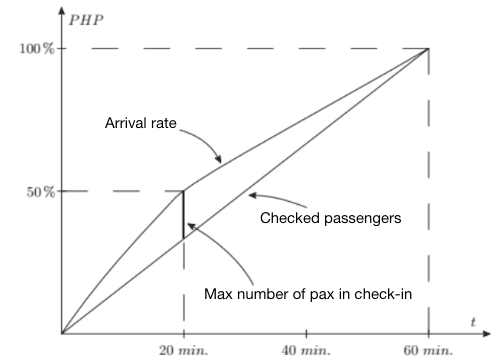
\includegraphics[width=10cm]{./images/graf1}
\caption{Plot PHP -- time.}
\end{figure}

Looking at the figure, it can be seen that the maximum number of checked-in passengers is 50\% in the first 20 min. Therefore:
\begin{align*}
\text{Fraction of total PHP} = \dfrac{PHP}{2}-\dfrac{PHP}{3}=\dfrac{PHP}{6}
\end{align*}

Therefore, the queueing area is of:
\begin{align*}
\textbf{Queueing area}=1.1\left( \dfrac{PHP+b}{6}s\right) \approx 700 \mathrm{m^2} = 750 \mathrm{m^2}
\end{align*}

Accounting for a security margin: Queueing area $= 750\mathrm{m^2}$.

The number of check-in counters must consider:
\begin{itemize}
\item Traffic characterized as international long-haul.
\item The average passenger load in the hour before and after the peak hour is 70\% of PHP.
\item Maximum queueing time (MQT) is 10 minutes.
\item Average time of check-in procedure (PTCi) is of 120 seconds.
\end{itemize}

We can compute the following factor:
\begin{align*}
X = \text{30-min peak at check-in} = PHP\cdot F1\cdot F2 = 2000\cdot 0.3\cdot 1.35 = 810
\end{align*}

Obtaining $F1$ and $F2$ factors from IATA tables:

\begin{figure}[ht!]
	\centering
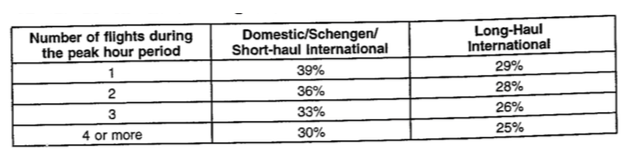
\includegraphics[width=8cm]{./images/IATA1}
\caption{F1: 30-min peak at check in as \% of PHP.}
\end{figure}

\begin{figure}[ht!]
	\centering
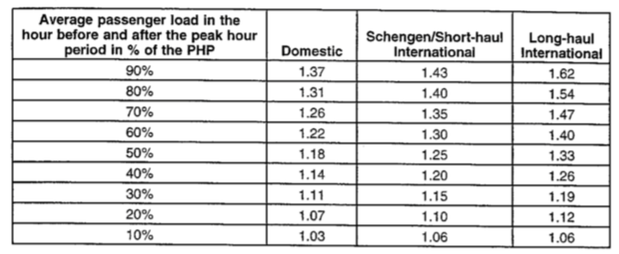
\includegraphics[width=8cm]{./images/IATA2}
\caption{F2: Additional demand based on previous and following flights to peak hour.}
\end{figure}

\begin{itemize}
\item MQT = 10 min (Maximum Queueing Time)
\item X = 810 (30-min peak at check in)
\end{itemize}

\begin{figure}[ht!]
	\centering
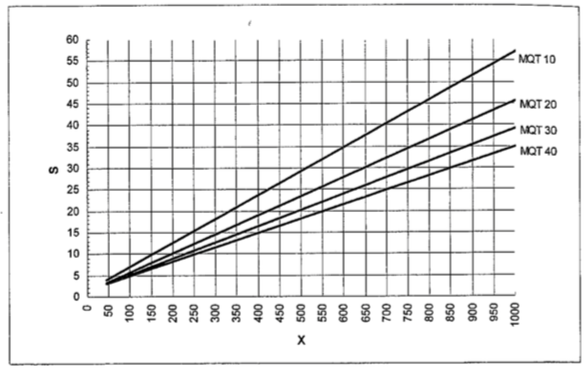
\includegraphics[width=10cm]{./images/IATA3}
\caption{Plot: S-X-MQT.}
\end{figure}

We can determine S as 49 check-in counters. Also we can add a 20\% for business class check-in counters.

\begin{align*}
\boxed{\text{\textbf{Total number of check-in counters}}= 59\text{ counters}}
\end{align*}

\item \textbf{Total passport control positions}: A multiple queue system will be used, having two accesses on each side, to reduce queues and passenger walking distances.

Considering:
\begin{itemize}
\item PHP(tot) $= 4000$ pax.
\item $b = 0 \hspace{2mm} \rightarrow$ connecting pax not processed in airside.
\item $t = 27\hspace{1mm}\mathrm{s}= 0.45\hspace{1mm}\mathrm{min} \hspace{2mm}\rightarrow$ average time per passenger in the process.
\end{itemize}

\begin{align*}
\boxed{\text{\textbf{Positions number}} = 1.1\dfrac{PHP+b}{60}\Delta t = 30}
\end{align*}

The total number of passport control positions will be 18. Since the ratio arrivals-departures is equal, the 50\% will be assigned to departures and 50\% to arrivals.


\item \textbf{Security controls:} To determine the number of x-ray machines needed, it is considered:
\begin{itemize}
\item PHP(dep) $= 2000$ pax.
\item $b = 0 \hspace{2mm} \rightarrow$ connecting pax not processed in airside.
\item $y = 600\hspace{1mm} \text{u/h} \hspace{2mm} \rightarrow$ number of units that the machine is able to process in one hour.
\item $y = 2\hspace{1mm} \text{units} \hspace{2mm} \rightarrow$ baggage items carried by passenger.
\end{itemize}

\begin{align*}
\boxed{\text{\textbf{X-ray machine number}}= \dfrac{PHP+b}{y}w = 6.666 \approx 7}
\end{align*}

A number of 7 x-ray machines are needed to give service to the airport.

\item \textbf{Health controls:} In the arrivals area, a health control is placed randomly for the passengers arriving from international flights. Considering:
\begin{itemize}
\item $t = 0.17\text{ min} \hspace{2mm} \rightarrow $ Average selecting process time.
\item $p = 400$ PAX $\rightarrow$ Number of PAX in the international critical aircraft (B777-300ER)
\item $m = 30$ min $\rightarrow$ required time to complete the control.
\end{itemize}

\begin{align*}
\boxed{\text{\textbf{Number of positions}} = \dfrac{p}{m}\Delta t \approx 3   }
\end{align*}


\item \textbf{Baggage claim area:} The dimensions of the baggage claim area, are compute according the following parameters.
\begin{itemize}
\item PHP(arr) = 2000 $\rightarrow$ arriving passengers per hour.
\item $w = 30$ min $\rightarrow$ average time per passenger.
\item $s = 1.8\hspace{1mm} \mathrm{m^2}$ $\rightarrow$ recommended area per passenger.
\begin{align*}
\boxed{\text{\textbf{Baggage claim area}} = 1.1\dfrac{aws}{60} \approx 1000 \hspace{1mm}\mathrm{m^2} }
\end{align*}
\end{itemize}

To compute the number of baggage claim belts, it is considered:
\begin{itemize}
\item $PHP$ = 1000 $\rightarrow$ arriving passengers per hour.
\item $q=0.7$ $\rightarrow$ proportion passengers in wide-body aircraft.
\item $r=0.3$ $\rightarrow$ proportion passengers in narrow-body aicraft.
\item $y=45$ min $\rightarrow$ average occupation time for wide-body aircraft.
\item $z=30$ min $\rightarrow$ average occupation time for narrow-body aircraft.
\item $n=400 \cdot 0.7$ min $\rightarrow$ number of pax in wide-body aircraft.
\item $m=200\cdot 0.3$ min $\rightarrow$ number of pax in narrow-body aircraft.
\end{itemize}

\begin{align*}
\boxed{\text{\textbf{Wide-body belts}}= \dfrac{PHP_2\cdot qy}{60n}\approx 4}
\end{align*}
\begin{align*}
\boxed{\text{\textbf{Narrow-body belts}}= \dfrac{PHP_2\cdot rz}{60m}\approx 5}
\end{align*}

The total number of baggage claim belts is 6. 

\item \textbf{Customs controls:} to determine the number of customs positions, the custom area needs to be defined.
\begin{itemize}
\item $PHP$ = 2000 $\rightarrow$ arriving passengers per hour.
\item $f=0.8$ $\rightarrow$  proportion of inspected passengers.
\item $s=1.5\hspace{1mm} \mathrm{m^2}$ $\rightarrow$ area recommended per passenger.
\item $t=2$ min $\rightarrow$ average passenger time.
\end{itemize}

\begin{align*}
\boxed{\text{\textbf{Number of customs positions}} = \dfrac{PHP\Delta f}{60}1.1\Delta t \approx 59}
\end{align*}





\end{enumerate}
\chapter{Structural typology description}
When it comes to building the terminal, it is important to specify which kind of materials are going to be used, and thus, the efforts that will hold the structure. In a general frame, it can be distinguished between two types of mechanisms of effort transmission to the foundation; firstly, the vertical efforts due to the gravitational load and, secondly, the lateral efforts due to the wind or possible earthquakes.

In the first case, the load-bearing elements work in compression and the ceilings work in bending-shear in the manner of a beam subjected to perpendicular loads in its plane.

In the second case, the same elements act differently. The ceilings receive and accumulate horizontal forces, working as a membrane and distributing forces between the different vertical elements, while the vertical elements work to bending-shear.

	\section{Foundation}
Indonesia is a country with a very varied terrain due to the numerous geological faults combined with significant erosion. Volcanoes are the spine of Java. This irregular chain of volcanoes, which spread over the entire length of the island, forms the most active part of the 'Ring of Fire' volcano chain. The volcanism typical of Java's Island corresponds to the alkaline series, in which basalts, tephrites and phonolites predominate. Moreover, the zone is full of subterranean activity, earthquakes are fairly common. Most of them are not very powerful but it is very important to take into account this phenomena in terms of building the foundations.

The Island of Java is a region located in a area close to the coast, which implies the abundance of swampy land. Therefore, a deep foundation will be carried out in front of a medium or superficial one, since the superficial terrain will not be able to absorb the efforts that will transmit through a direct foundation.

Once selected the deep foundation method, it is proceed to define the geometry of the piles with which this foundation will be done. The piles to be used will be cylindrical and the relationship established between its height (H) and radius (R) in order to assure the consistency of the foundation is the following one:

\begin{equation}
\frac{Height}{Radius}>15
\end{equation}

Usually, the height values of the piles will not exceed the 40 meters. From a conservative point of view, it has been selected a height of 35 meters and a base of radius 2.25 meters, which corresponds to a H/R factor of 15.55.

The last step to finish the foundation is to decide whether they are constructed with in situ piles or pre-fabricated ones. In the first case, piles in situ are better than the others in terms of acoustic pollution produced during its installation, but when it comes to low quality construction terrains it can not be the best solution. On the other hand, and therefore the remaining option, is the use of prefabricated piles, which are placed directly. The inconvenience is that this system requires the transport of the previously built piles to the site in which the foundation will be done. Moreover, it is important to take into account the very intense noise and vibrations this process will produce. Although the mechanism of intrusion of the piles by pressure is not suitable for all types of terrains, it is the appropriate method to build the foundations due to the characteristics of the region.

\begin{figure}[H]
	\centering
	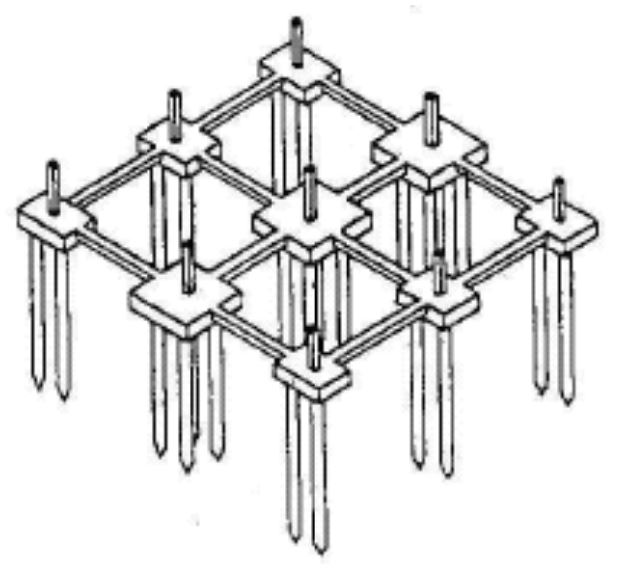
\includegraphics[clip, trim=0cm 0cm 0cm 0cm, width=0.4\textwidth]{./images/TipologiaEstructural/foundationprefabricated}
	\caption{Schema of deep foundation with prefabricated piles.}
	\label{foundation}
\end{figure}

	\section{Vertical elements}
The pillars are the resistant elements responsible for supporting mainly compression loads in a vertical direction and also can absorb small lateral bending loads. The main function of them is to distribute the loads of the ceiling and the slabs to the foundation. It is important to remark that there is an alternative of vertical resistant elements, which are the loading walls but in case of Bekasi-East Jakarta Airport this solution will not be carried out.

The basic types of pillars found in construction are in situ reinforced concrete, prefabricated concrete, metal structure and mixed structure of steel and concrete. In the case of the new airport's terminal building, it is decided to make the pillars with mixed structure of steel and concrete. In this way, the pillars will have smaller sections than the those made of in situ reinforced concrete and will have more fire resistance than the metallic ones. Moreover, this type of pillars work very well in front of earthquakes, since the metallic armor is able to support the efforts in order to maintain the building up.

Starting from the foundation, the pillars of the ground floor will have a considerable section, since they will have to support greater loads and  weight of the structure.

As far as the upper floor is concerned, some of the pillars from the ground floor will be extended to this level. At the level mentioned, it will not be necessary to place the same number of pillars as in the ground floor, since the structure in this case has to support less efforts and weight.

The distribution of the pillars can be seen in the drawings of the airport attached to the documents.

	\section{Slab}
The slab is the horizontal structural element that directly receives the loads and transmits them to the remaining elements of the structure. Before deciding what type of slab will be used in the terminal building it is necessary to know the
functions of it:

\begin{itemize}
		\item Support itself and the loads received
		\item Support the construction process
		\item Solidarize all the elements of the plants
		\item Distribute the horizontal loads between all the elements
		\item Present compatibility of deformations with their functions
		\item Isolate the plants thermally and acoustically
		\item Resist to fire
\end{itemize}

It is also important to differentiate between types of slabs. It can be found unidirectional slabs, usually prefabricated or made of beams and vaults, and bidirectional, which can be waffle slabs or solid slabs.

Having a look to these different types of slabs, it is decided that the best option to the new airport terminal building will be a bidirectional waffle slab which will provide a bi-dimensional loads distribution. They are flat slabs without beams, composed of nerves in two directions, which can be built with recoverable moulds or with permanent lightening. The waffle slab must be filled with reinforced concrete and later framed. This process implies the need of approximately 28 days to be ready. The waffle frame allows to have higher lights than other ones and, in addition, there is no problem concerning its transportation, since it is built using in situ reinforced concrete.

\begin{figure}[H]
	\centering
	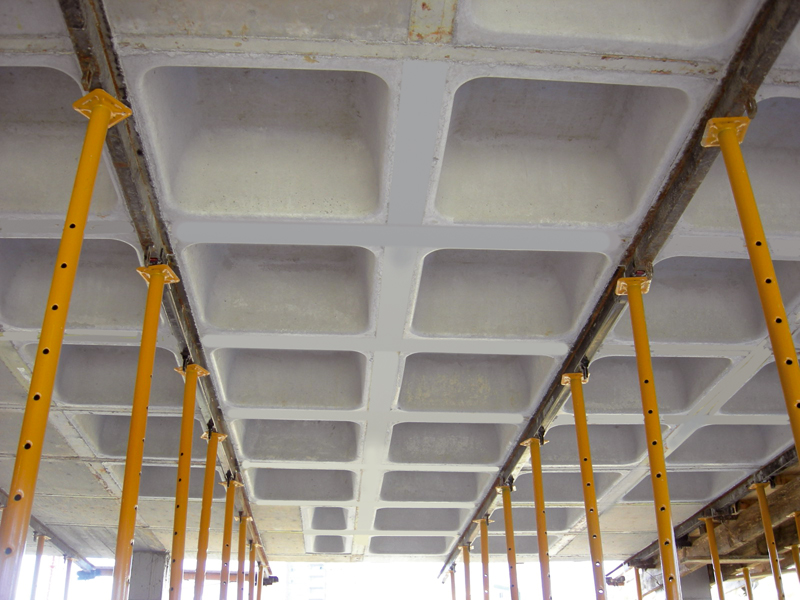
\includegraphics[clip, trim=0cm 0cm 0cm 0cm, width=0.5\textwidth]{./images/TipologiaEstructural/waffleslab}
	\caption{Example of bidirectional waffle slab.}
	\label{slab}
\end{figure}



	

\chapter{Indoor flooring}

	\section{flooring typology}
	
	Indoor flooring or paving is the horizontal base of a building (or the different bases of each building level). It works as a support for people or furniture. Indoor paving can be provided with several types of coating (wood, ceramics, marble, et cetera).
	
	The coating material is the first thing to be decided before choosing any other feature of the floor, such as color, texture or specific details.
	
	In general, the most common used materials in flooring are: wooden floors, ceramic floors, petrous floors and those made of concrete. There are also other materials, such as metallic and artificial composite floors, although these are less common.
	
	Depending on the application that is going to be given to the floor, or the indoor zone in which is going to be set up, one must take into account the following aspects:
	
	\begin{itemize}
	\item \textbf{Wear and tear resistance}: it is advised to use ceramic floors, petrous or concrete. For example, in circulation areas or stairs.
	
	\item \textbf{Perforation resistance}: some concretes with specific resistances, some petrous or ceramic floors. 
	
	\item \textbf{Humidity resistance}: ceramic, petrous and ceramic offer a high humidity resistance; on the other hand, wooden floors are not recommended. To be taken into account in restrooms or rainy areas.
	
	\item \textbf{Resistance to chemicals}: some kind of petrous floors such as granite and specific ceramics. In zones where chemical pourings can happen.
	
	\item \textbf{Hygiene}: the floor must have the ability of being easily cleanable and waterproof, to show an attractive and newflanged aspect.
	\end{itemize}
	
	To back up the decision that has been made, some general features of each floor type are presented next:
	
	\begin{itemize}
	\item \textbf{Wooden floors}: 
	Nowadays, and thanks to the advanced wood treatments, it is possible to find dyed and varnished wooden floors. These kind of floors can last up to 50 years. They add warmness to cool places; and with a proper setting and maintenance they can remain as untouched during several years. Among their disadvantages, it is found that they require special care for cleaning and mantaining and also they can be deteriorated with humidity or water pouring. Wooden floors can be natural, synthetic or laminated. These floors are more common in Europe.
	
	\item \textbf{Ceramic stoneware or porcelain stoneware floors}:
	These kind of floors have a decent price according to its usage. The average lifetime of a stoneware tile is of about 30 years. Naturally, they have low resistance to wear due to material properties, although the can be restructured to increase resistance.
	
	\item \textbf{Petrous floors}: 
	Different kind of stones are used in flooring: marble, slate, granite, quartz, sandstone, etc. Their main advantage is the wear resistance. This resistance is greater than for ceramic stoneware floors. Due to the attractive patterns and high resistivity properties, these materials can be the most expensive.
	
	Regarding marble pavings, this material denotes nobility and it was usually used for paving prestigious places. Its main features are its aspect and resistance; its disadvantages are the coldness to touch, and the necessity of a high maintenance to avoid imperfections.
	
	Other rocks used in paving are quartz, slate and granite, being the lattest much resistant than marble, but very expensive to cut, prepare and set into the floor.
	
	\item \textbf{Vinyl floors}:
	Vinyl floors are easy to clean, they also resist humidity and water pourings. They are easy to replace and to set above other floor coatings. This kind of floors are thermic and electrical insulators. Among their disadvantages, they look artificial and need a careful and correct use to avoid imperfections.
	
	\item \textbf{Smooth concrete floors}:
	This kind of floors are easy to maintain and offer resistance. Drawings, shapes and colors can be designed on it. A proper instalation leads not only to a good appearance but also to a greater resistance avoiding wear and fissures.
	
	\item \textbf{Brick floors}:
	Brick floors are economic, providing a rustic decoration or also common in exteriors, they offer a high sensitivity to attrition and show wear in heavily-transited areas.
	
	\item \textbf{Carpet floors}:
	They are quite economic and of easy instalation, without the need of hiring specialized personnel. Like wooden floors, carpet is available in different colors and patterns and provides warmness, and add aesthetics in the place used. It insulates sound and temperature. Its main disadvantage is the accumulation of dust, and therefore it requires a constant maintenance. Carpet floors are very common in the U.S., specially in public places such as airports.
	\end{itemize}
	
	\section{Floor covering}
	
	In any paving, before setting the upper finishing layer, which is different depending upon the zone, it is important to know the layers that have to be included in-situ:
	\begin{itemize}
	\item Surface layer 
	\item Grip layer 
	\item Leveling layer 
	\item No-grip intermediate layer 
	\item Structural base 
	\end{itemize}
		\subsection{Structural base}
	The structural base is the layer that lies onto the floor. In the particular case of indoor paving, it is formed by a ground slab.
	
	Ground slabs, also knowns as floor framings, are classified in terms of stability as a consequence of hydraulic retention, according to the normative UNE 22202-1.
	
	The thickness of the ground slabs is determined by means of structual criteria, as functions of the CBR (California Bearing Ratio). On the other hand, a solicitation computation is also required.
		\subsection{No-grip intermediate layers}
		
	To enhance the floor properties different layers composed by different materials are inserted. These layers are the following ones:
	\begin{itemize}
	\item Waterproof layer: this layer raincoats the floor against liquid water. It is recommended to use a polyethylene layer of a minimum thickness of 2mm. 
	\item Drainage layer: it helps removing the water that might be stored by means of a small slope. 
	\item Acoustic insulation: there are specific layers for this function, and it helps insulate and reduce the impact of aerial noise, which is spread within the structure.
	\item Thermal insulation: it enchances a greater thermal resistance.
	\end{itemize}
		\subsection{Leveling layer}
	These kind of layers are used to achieve the required flatness of the firm, and if a certain slope is required, they also provide this slope.
		\subsection{Grip layer}
	It consitutes the union between structural base and the tile or coating. It can be made of a leveling mortar or an adhesive. In the project, a leveling mortar has been chosen.
		
	\section{Design}
	The floor design and aesthetics is wanted to produce a homely and cozy feeling. In order to do so, it has been thought that it could fit with the tonalities of the landscapes that can be seen all across the country, and the beautiful sceneries that are spread along the islands and towns of Indonesia.
	
	There is a lot of culture of esculptures in the islands of Java and Bali, for this reason, a floor design that reminds of the ancient sculptures of the country could fit in the airport and also provide a clean, elegant and cozy appearance.
	
	\begin{figure}[ht!]
	\centering
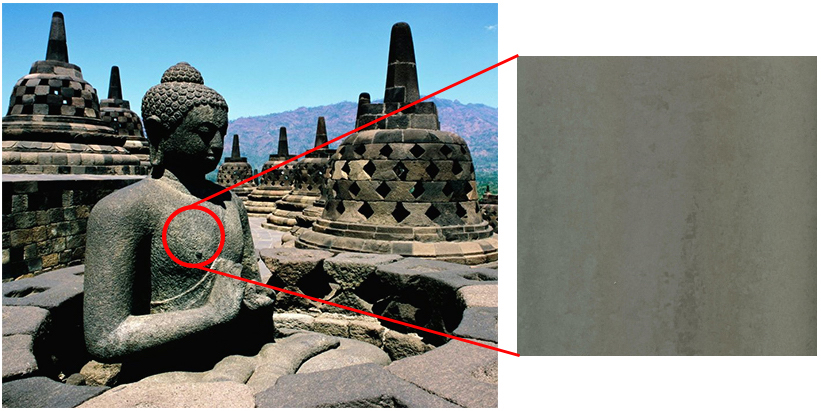
\includegraphics[width=13cm]{./images/SueloGeneral}
\end{figure}

On the other hand, an inspiration from the beautiful and relaxing beaches that the country offers, it has been chosen a floor that reminds of the sand that one can find in these beaches.

\begin{figure}[ht!]
	\centering
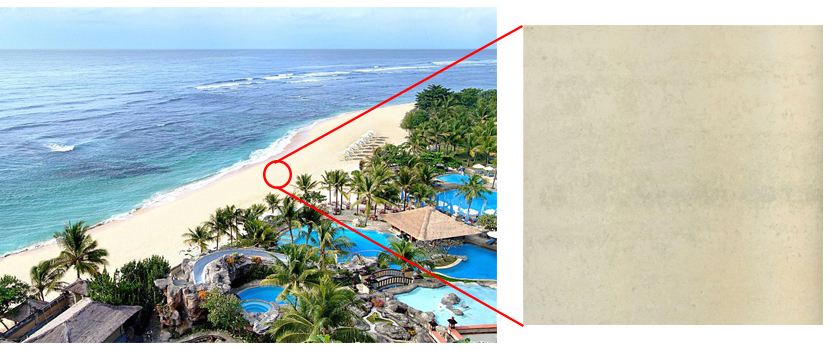
\includegraphics[width=15cm]{./images/SueloSecundario}
\end{figure}

	
	
	
	\section{Superficial layer}
		\subsection{Common areas flooring}
	In the common areas, it has been chosen to use a ceramic porcelain stoneware Floor Gres material, in particular the technical strong collection Chromtech/1.0 from the Floor Gres company, that is suitable for heavy traffic areas thanks to its high resistance. The color will be a neutral grey named cool/3.0 in the Floor Gres company color gamma.
	
	\begin{table}[ht!]
	\centering
	\begin{tabular}{|c|c|c|}
	\hline
	Specification & Normative & Value\\
	\hline
	Water Absorption & ISO 10545-3 & $<0.1\%$\\
	\hline
	Breaking Strength & ISO 10545-4 & $>1700$ N\\
	\hline
	Scratch Hardness & ISO 10545-6 & $< 150 \mathrm{mm^3}$\\
	\hline
	Thermal Shock Hardness & ISO 10545-9 & Resistant\\
	\hline
	Chemical Resistance & ISO 10545-13 & UA ULA UHA\\
	\hline
	Coefficient of Friction & DIN 51130 & R10 (Matte)\\
	\hline
	\end{tabular}
	\caption{Technical Specs of Floor Gres Chromtech/1.0 floor.}
	\end{table}
	
The color chosen for our tiles within all the color shades is the one known as "Cool 3.0" with a matte and polished finishing.
	\begin{figure}[ht!]
	\centering
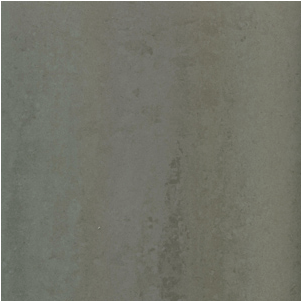
\includegraphics[width=1cm]{./images/Color}
\caption{Neutral gray color (Cool 3.0) from Floor Gres gamma.}
\end{figure}

The result of the floor chosen in the common areas is the following:
\begin{figure}[ht!]
	\centering
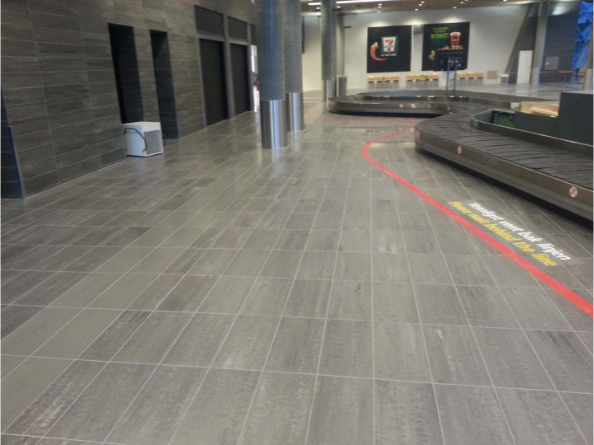
\includegraphics[width=10cm]{./images/Resultado}
\caption{Result of instaling Chromtech/1.0 tiles in common areas.}
\end{figure}
		\subsection{Stairways and secondary areas flooring}
	Due to the high-end properties provided by the floor used in the common areas, it has been decided to use the same material but with a different tonality. In this case, the color chosen is  a beige/taupe named Cool 1.0 in the Floor Gres color gamma. It is provided with a matte finishing.
	
	The technical specs of these tiles are the same as for the tiles used in common materiales provided that the only change is the color. In general, this product provides an excellent finishing and it offers a high resistance. For this reason, it can be used in heavily-trafficked areas.
	
	The color that has been chosen for stairways and secondary areas such as VIP lounges is the following:
		\begin{figure}[ht!]
	\centering
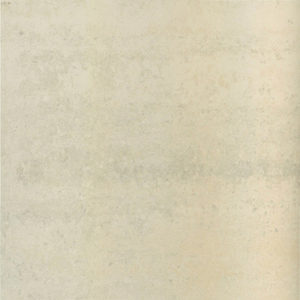
\includegraphics[width=1cm]{./images/Color2}
\caption{Beige/taupe color (Cool 1.0) from Floor Gres gamma.}
\end{figure}

The result of the floor chosen in stairways and secondary areas is the following:
\begin{figure}[ht!]
	\centering
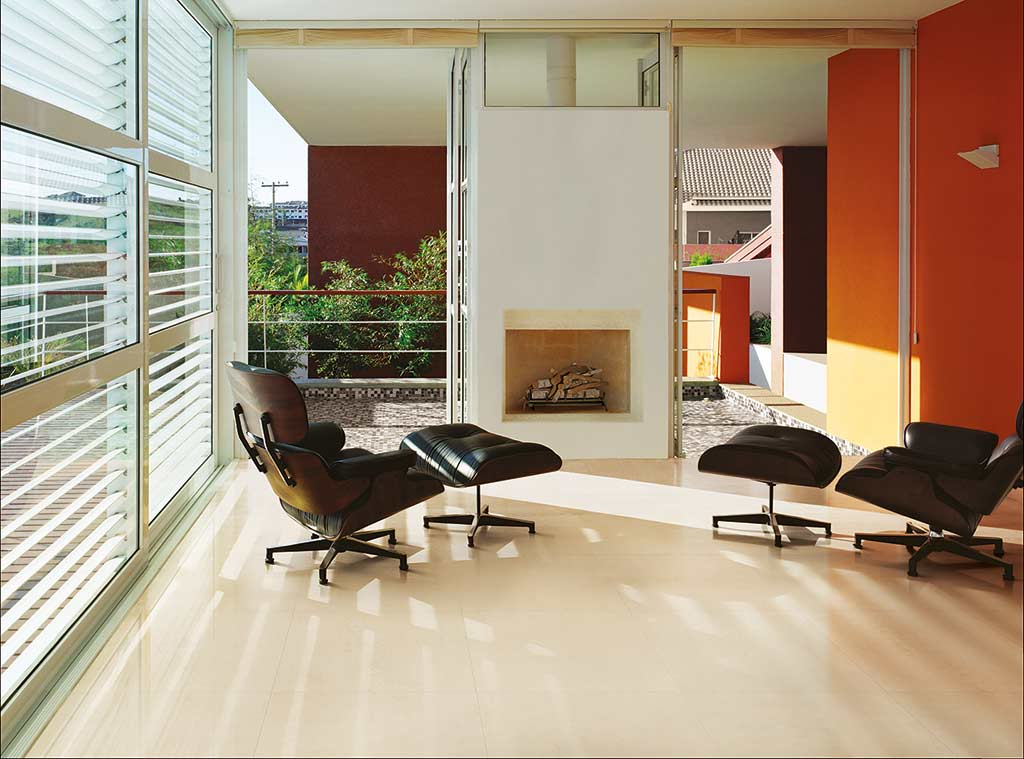
\includegraphics[width=10cm]{./images/Resultado2}
\caption{Result of instaling Chromtech/1.0 tiles in secondary areas.}
\end{figure}
		\subsection{Restrooms flooring}
	For the restrooms paving, it has been decided to use a rectified porcellanato tile, named "Portland Caliza" from the Spanish company Porcelanosa. These tiles are provided with anti-slip properties, making them exceptional for the usage in restrooms.
	
	The color chosen is called "colored biscuit" and it is a neutral light gray:
			\begin{figure}[ht!]
	\centering

\includegraphics[width=1cm]{./images/Color3}
\caption{Neutral light gray "Colored Biscuit" from Porcelanosa.}
\end{figure}

The result of instaling these tiles in the airport restrooms is the following:

\begin{figure}[ht!]
	\centering
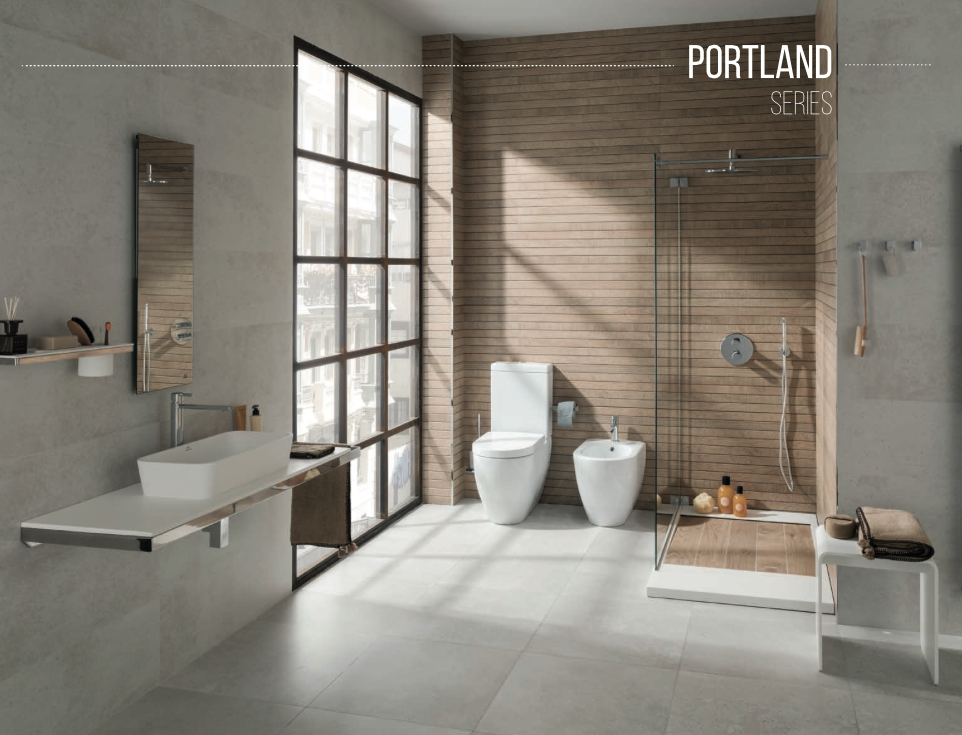
\includegraphics[width=8cm]{./images/Resultado3}
\caption{Result of instaling Portland Caliza tiles in restrooms.}
\end{figure}
	
		\subsection{Offices flooring}
	The airport offices for ANSPs, customs and airlines are going to be provided with a porcelain stoneware tile called Basalike from a company called Panaria. The supply of these tiles is to be provided by the Italian company Sognando Casa, that manufactures several types of materials for indoor flooring.
	
	These tiles offer an excellent natural finishing with an antislip index R10. The color chosen is a dark gray that inspires calmness and make the offices the perfect spot for working in any season of the year.
	
	The color that will be instaled in the offices floor is the following:
\begin{figure}[ht!]
\centering
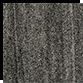
\includegraphics[width=1cm]{./images/Color4}
\caption{Dark gray color in Basalike tiles from Panaria company.}
\end{figure}

The result of instaling these tiles in the airport offices is the following:
\begin{figure}[ht!]
	\centering
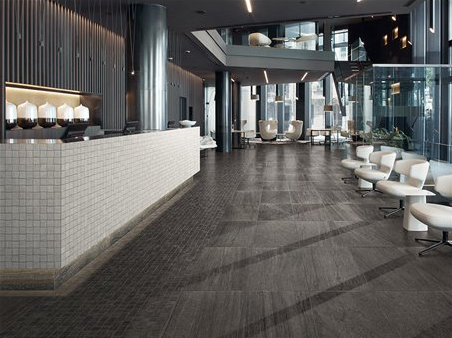
\includegraphics[width=10cm]{./images/Resultado4}
\caption{Result of instaling Basalike tiles in the airport offices.}
\end{figure}

These tiles have good quality and are optimum for an office flooring. In the next table, the technical specifications are shown:

	\begin{table}[ht!]
	\centering
	\begin{tabular}{|c|c|c|}
	\hline
	Specification & Normative & Value\\
	\hline
	Water Absorption & ISO 10545-3 & $<0.5\%$\\
	\hline
	Breaking Strength & ISO 10545-4 & $>1300$ N\\
	\hline
	Scratch Hardness & ISO 10545-6 & $< 175 \mathrm{mm^3}$\\
	\hline
	Chemical Resistance & ISO 10545-13 & LA, HA\\
	\hline
	Coefficient of Friction & DIN 51130 & R10 (Natural)\\
	\hline
	\end{tabular}
	\caption{Technical Specs of Panaria Basalike floor.}
	\end{table}
	
		\subsection{Automatic baggage handling system flooring}
		
	The automatic baggage handling system flooring is not so much sophisticated and for obvious reasons, ceramic or porcelanic tiles will not be used. In this area, polished concrete is to be used since it provides a set of good properties for this application:
	\begin{itemize}
	\item High surface mechanical resistance.
	\item Greater useful life than conventional concrete.
	\item High density and low porosity.
	\item Easiness of maintenance and cleaning.
	\item Low dust formation.
	\end{itemize}
The supplying of the concrete and its respective polishing will be provided by the Spanish company EIROS, since it offers a good service at a honest price.

\begin{figure}[ht!]
	\centering
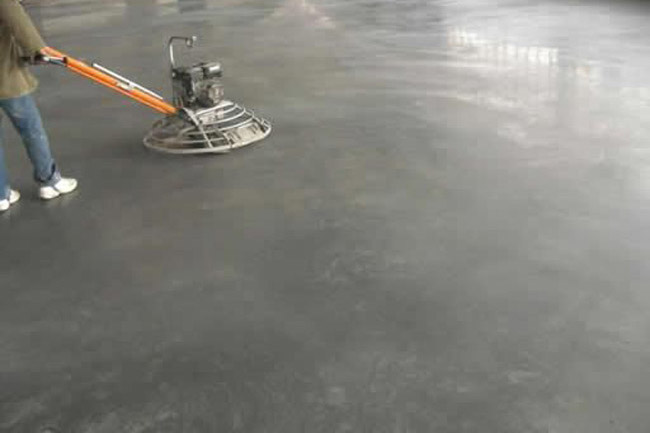
\includegraphics[width=10cm]{./images/Resultado5}
\caption{Result of instaling polished concret in the ABHS system (SATE).}
\end{figure}

		
\chapter{Facade}

In this chapter, the terminal building facade is going to be designed. To do so, different aspects and issues have been accounted such as: building location, solar incidence, among other factors.

Apart from the aspects that mainly constitute the facade, all the facade-integrated elements will be decided such as doors, windows and access gates. 

	\section{Front, back and dock facades}
		\subsection{Requirements and adopted solution}
		
It has been decided to use a glass facade for several reasons. Apart from current trends and fashions, the reasons why it has been chosen are:
\begin{itemize}
\item \textbf{Providing a calming feeling to the passengers}: glass facades allow to see through them, enabling the passengers to see the take-offs and landings, making them lose fear and providing a relaxing feeling.
\item \textbf{Increasing luminosity}: the glass facade increases luminosity naturally lighting the interior of the building during day-time hours. Sometimes, excessive sun incidence can be a disturbing factor that has to be studied and managed properly.
\item \textbf{Providing a spacious enclosure}: the usage of glass facades increases the spacious feeling, being favorable for passengers and employees and thus, avoiding cramped enclosures.
\item \textbf{Aesthetic reasons}: glass facades are modern and provide a beautiful innovative aspect from inside and outside. Furthermore, glass can be highly customizable (opacity, brightness, reflective...) allowing multiple design solutions.
\end{itemize}

The usage of glass facades is constrained by some rules that have to be fulfiled:
\begin{itemize}
\item \textbf{Safety}: in order to avoid that glass breaks or falls apart, it must be used laminated glass (sheet glass). This kind of glass, additionally offers a high protection against UV rays, filtering up to 99\% of them.
\item \textbf{Thermal insulation}: since the facade is an exterior element, it is important to account the thermal insulation. It is highly recommended to use double layered glazing to avoid heat loss, reduce heating consumption and increase comfort.
\item \textbf{Acoustic insulation}: greater or lesser thicknesses or camera widths (in double layered glazing) are to be defined to improve acoustic attenuation.
\item \textbf{Mechanical issues}: depending upon the loads and solicitations, the thicknesses will be greater or lesser.
\end{itemize}

Glass facades present several typologies. In order to justify why it has been chosen one or another, the main four types are going to be presented next:
\begin{itemize}
\item \textbf{Curtain wall}: this system is used in small-medium magnitude. Glass is installed in front of slabs, and it provides a complete closing, giving a modernity aspect.
\item \textbf{Ventilated facade}: glazing system in which a double skin is applied on a curtain wall. 
\item \textbf{Windows closure}: this system is instaled between slabs. It allows to obtain a quick closing of closures, since each level is independent from the others. It is not necessary using firewalls between slabs, because there is no contact point between two closures.
\item \textbf{Spider system}: in this system, the support is provided by stabilizing connectors such as tensioners, glass ribs or steel pillars, that are adhered to the glass surface by means of structural fittings called "spiders".
\end{itemize}

	\begin{figure}[ht!]
	\centering
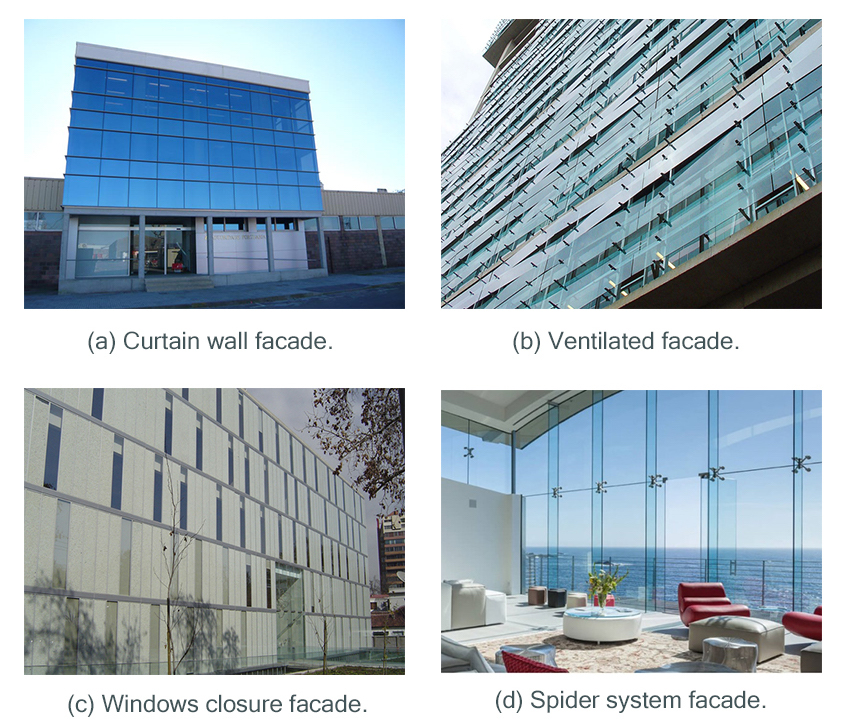
\includegraphics[width=11cm]{./images/Facade/facades}
\caption{Glass facades typologies.}
\end{figure}

Due to the building complexity and the beautiful finishing design, it has been chosen to use a spider system facade. Within this type of facades, there are three different types depending upon the structural fittings that are used: glass ribs, steel pillars or tensioners.

	\begin{figure}[ht!]
	\centering
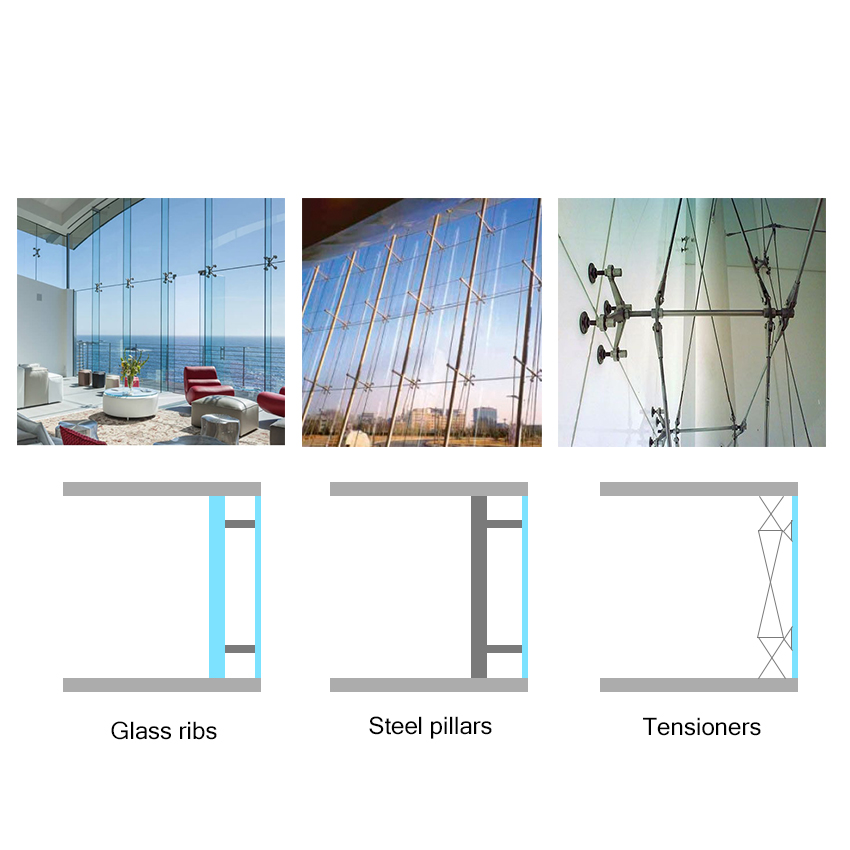
\includegraphics[width=11cm]{./images/Facade/spiders}
\caption{Spider glass system typologies.}
\end{figure}

According to the building characteristics, it has been decided that the spider glass fittings will be steel pillars. The other systems would be too expensive given the dimensions of the building and would become the structure much complex.



		\subsection{Glass}
	The glass to be used is in charge of the SunGuard company. This company recommended to use the Guardian SunGuard Extra Selective SNX 60 glass. It is one of the best products of solar control glass avilable in the current industry.
	
	The SNX 60 has an attractive, uniform, neutral and transparent appearance, regardless the angle of vision. The internal color reflexion has been optimized, allowing a more neutral color tone when it is seen from the inner part of the building. 
	
	This glass, allows the incidence of 60\% of neutral light and only 29\% of solar heat. It is leader in the market for being one of the products with higher selectivity (ratio between light transmission and solar factor). SNX 60 is available in annealing version (recocido) or temperable. Below, one can find a table with the main characteristics of the selected glass:
	
\begin{figure}[ht!]
\centering
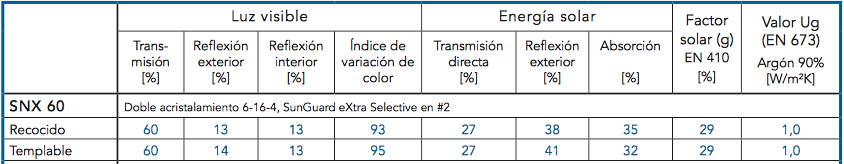
\includegraphics[width=15cm]{./images/Facade/performances}
\caption{Selected glass characteristics (SNX 60).}
\end{figure}

For illustrative purposes, the glass chosen would look as follows in the building:

\begin{figure}[ht!]
\centering
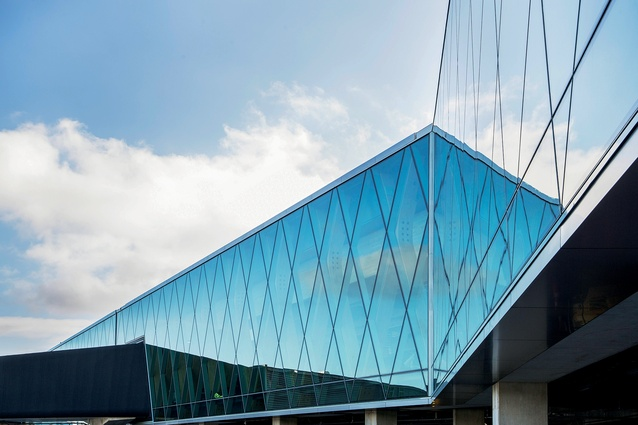
\includegraphics[width=13cm]{./images/Facade/snx60}
\caption{View of a building made of SNX 60.}
\end{figure}

	
	
		\subsection{Spider system with steel pillars}
	The Spider system has been contracted to the German GLASSCON company. They offer all the fittings system for anchoring the glass. The chosen solution has been: Steel supporting solution type "GL/SSS". In this case, only steel pillars would be used, tensioners are not necessary.
	
	\begin{figure}[ht!]
\centering
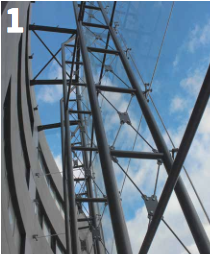
\includegraphics[width=6cm]{./images/Facade/steel}
\caption{Steel supporting solution type "GL/SSS" (GLASSCON).}
\end{figure}
	
		\subsection{Steel and concrete mixed columns}
	Mixed columns are a combination of concrete columns and steel columns, joining advantages from both types of columns. Mixed columns have a greater ductility than purely concrete ones; also, fittings and unions can be built using steel construction techniques. The concrete filling not only provides a greater capacity for supporting loads but also increase the fire resistance.
	
	Different profiles are used for mixed columns. It has been decided to use tubular columns for aesthetical reasons and for the following reasons:
	
\begin{itemize}
\item Concrete filling provides greater stiffness and greater ability of supporting loads in tubular columns. Therefore, aesthetic and thin columns can support large loads without increasing external dimensions.
\item Tubular design is useful for concrete framing and reinforcement.
\item No necessary extra equipment is needed for concrete filling in the tubular design rather than the equipment used in usual concrete works.
\end{itemize}
	
		\begin{figure}[ht!]
\centering
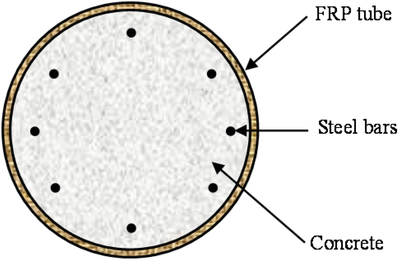
\includegraphics[width=5cm]{./images/Facade/columns}
\caption{Mixed steel and concrete tubular column.}
\end{figure}

In-situ concrete will be provided by the company PT Hume Concrete Indonesia, located a few miles away from the airport location. Tubular steel pillars will be provided by another Indonesian company called Mittal Steel Company.

The columns will be used for supporting the building cover and will have a thickness (diameter) defined by the the structural design team.
	
	
	\section{Secondary areas facade}
		\subsection{Facade (prefabricated concrete)}
	The secondary areas facades of the building, which do not have any aesthetical requirement (since it is where the ABHS (SATE) system, offices and handling dependencies will be allocated) are decided not to be made of glass. 
	
	Several necessities need to be fulfiled, for instance, privacity of the offices but always trying to search for an attractive appearance for the people who will work there. 
	
	For this reason and also for its insulation properties, prefabricated concrete has been decided for closures in the lateral facade including elements such as doors, gates and windows where required.
	
	This material is based on large concrete panels formed in the factory, for this reason, its shapes and dimensions are standardized. The option of providing thermal insulation is available and they can be used either in vertical or horizontal orientation. Another advantage is that they do not need surface finishings since these are included in the forming, as a consequence are aesthetically attractive. The biggest disadvantage is that the structures are heavy and they need a good base structure to make the anchorage.
	
	Other advantages of this structure are: high resistance, clean work, high availability, high durability, excellent fire resistance properties, relatively low price with respect to traditional facades.
	
	The panels are made of architectonic concrete, namely, they are steel-armed concrete. Variable dimensions, thicknesses (from 8cm) and weights are available. These panels have the following features:
	\begin{itemize}
	\item Supporting structures (they are part of the building structure transmitting mechanical stresses to the ground or foundation.
	\item Preformed multilayer with thermal insulation. The insulation material that they contain is expanded polystyrene.
	\end{itemize}

The companies offer prefabricated panels, with a special design to include windows or doors inside.

The company that will provide these prefabricated concrete panels will be Hormipresa S.A., that is leader in its sector having carried out a wide range of projects of all kinds.

Next, the dimensions, properties and features of the slabs (panels) to be instaled are presented:

\begin{table}[ht!]
\centering
\begin{tabular}{|c|c|c|c|c|}
\hline
\vtop{\hbox{\strut Weight} \hbox{\strut [kN/$\mathrm{m^2}$]}} & \vtop{\hbox{\strut Length (L)} \hbox{\strut [m]}} & \vtop{\hbox{\strut Thermal ins.}  \hbox{\strut [kcal/h C $\mathrm{m^2}$]}} & \vtop{\hbox{\strut  Acoustic ins.}  \hbox{\strut [dbA]}} & \vtop{\hbox{\strut Fire resistance} \hbox{\strut [Ei-min]}}\\
\hline
4.00 & 12 & 0.43 & 53.5 & 120\\
\hline
\end{tabular}
\caption{Properties and features of the instaled panels.}
\end{table}

The rectangular slabs will have the following dimensions:
\begin{itemize}
\item Longitude (L): 12 m
\item Longitude (w): 3 m
\item Thickness (e): 2 m
\end{itemize}

Nevertheless, a set of slabs of specific measures will be ordered for areas where the design needs a different kind of measures rather than the standard ones. 

Another issue to be defined is the surface finishing that the lateral facade will have.

	\begin{figure}[ht!]
	\centering
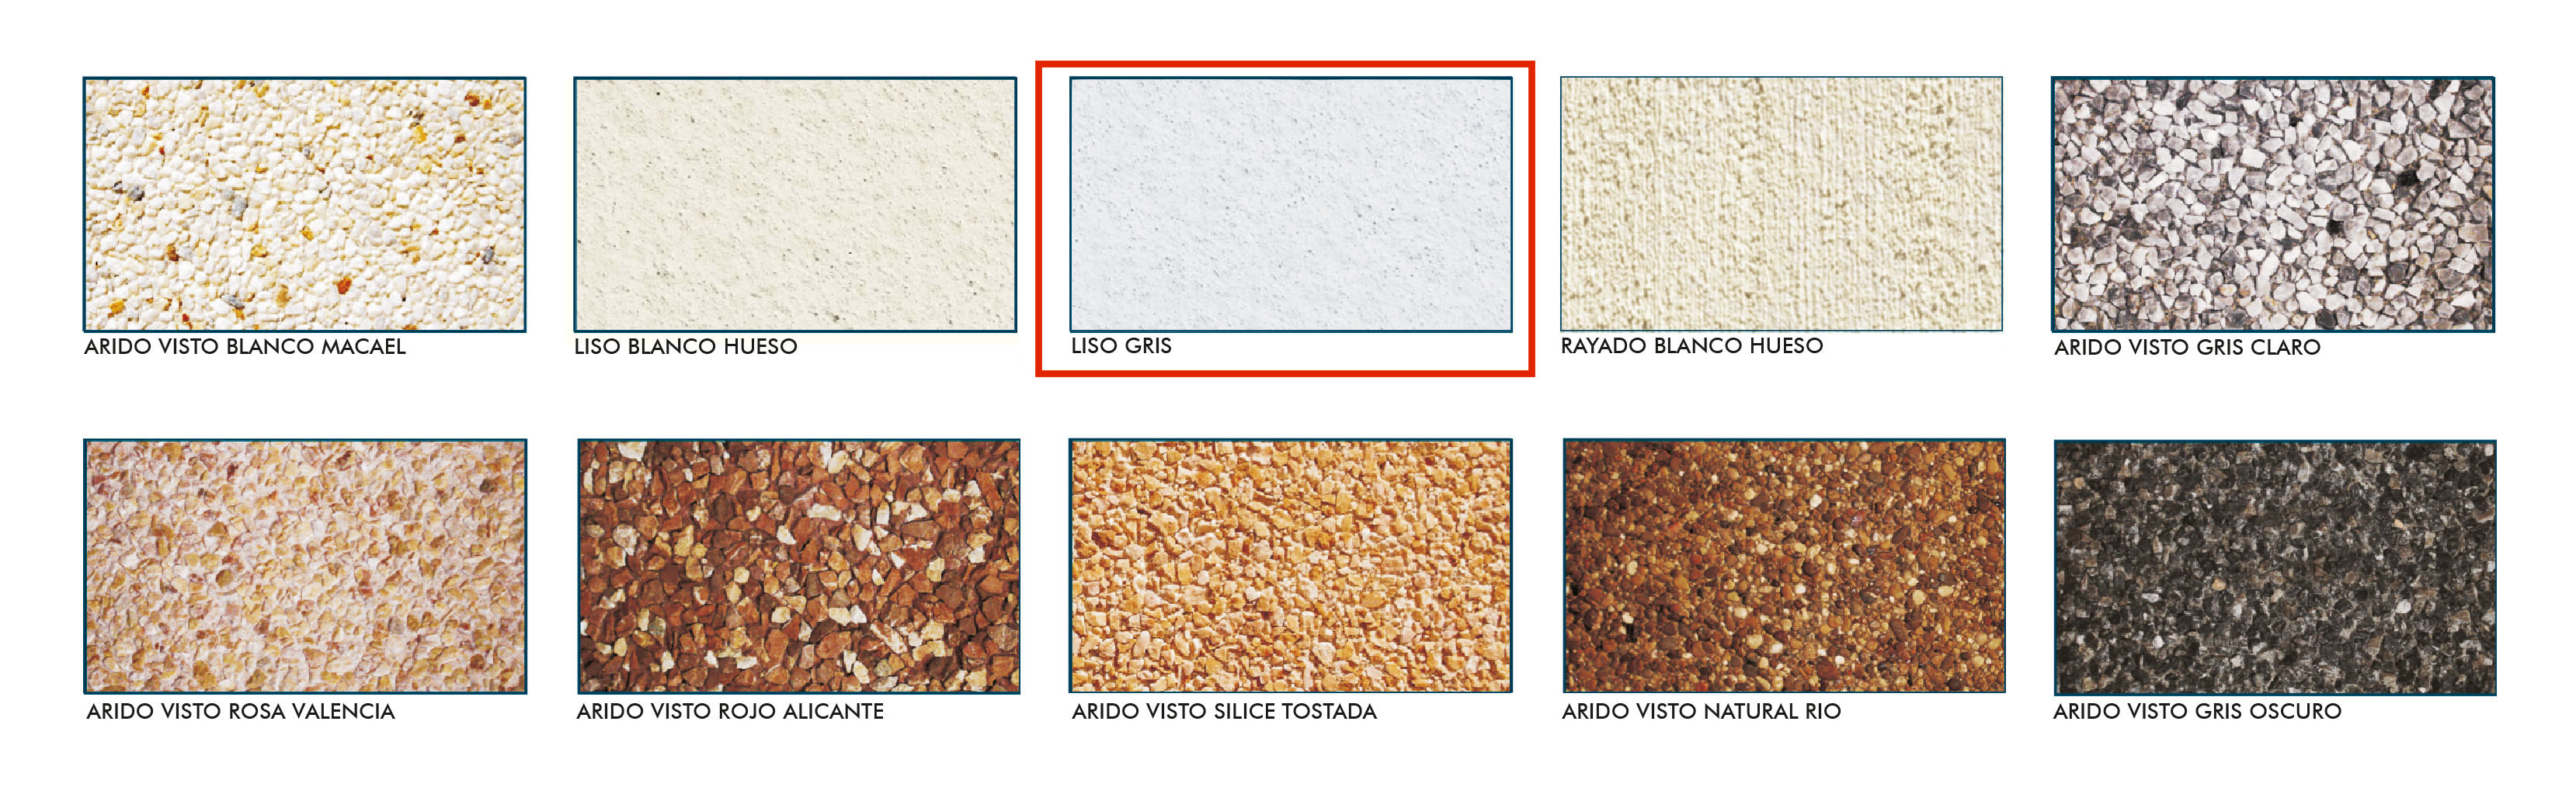
\includegraphics[width=13cm]{./images/Facade/finishing}
\caption{Surface finishing catalogue.}
\end{figure}

The selection has been the smooth gray color, from the catalogue above. Within this possibilities, and taking into account the design of the terminal building it has been decided that this color is which suits the best. The secondary areas facades will be connected with the glass facade described in the previous section.




	\section{Other elements}
		\subsection{Main doors}
	Due to the large dimensions of the terminal building and multiple accesses, there are 4 main entrance and 4 main exit revolving doors in the terminal building. The provider company is GEZE established in Germany.
	
	The door model to be used are GEZE fully-automatic revolving door TSA 325 NT, which has an interior diameter of 3600mm.
	
	The main features of this product are:
	\begin{itemize}
	\item They are activated by a motion detector inside and out.
	\item Adjustable automatic speed, the run out time can be freely set to "summer" mode (longer) or "winter" mode (none). In order to avoid heat loss.
	\item Optional disabled button can be used to reduce the rotation speed and to ensure easy access for wheelchair operators or persons with limited mobility.	
	\item Type-approved according to DIN 18650 and certified.
	\end{itemize}
	
		\begin{figure}[ht!]
	\centering
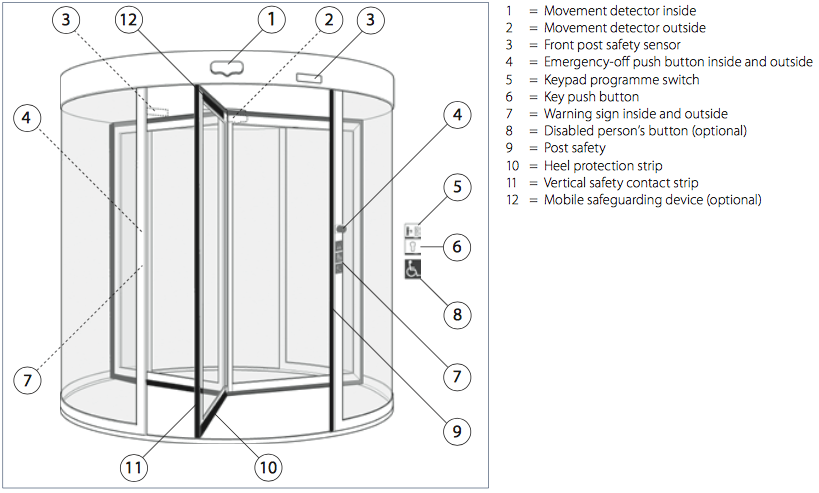
\includegraphics[width=13cm]{./images/Facade/scheme}
\caption{Revolving door selected for terminal building main entrances and exits.}
\end{figure}

For illustration purposes, the result of using these revolving doors in the terminal building would be:

		\begin{figure}[ht!]
	\centering
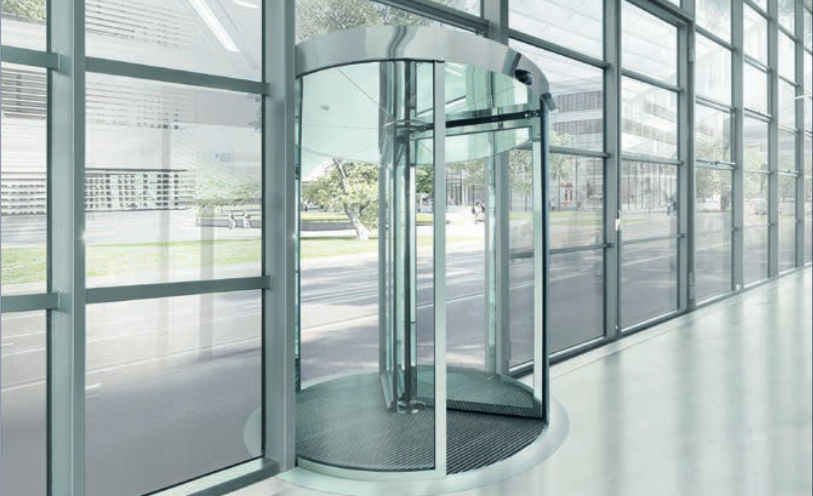
\includegraphics[width=13cm]{./images/Facade/revolving}
\caption{Revolving door selected for terminal building main entrances and exits.}
\end{figure}
	
	
		\subsection{Access bridges}
	Access bridges between terminal and jetway (gangway to the aircraft) are the connecting structures between the jetways to access the aircraft and the terminal building. Due to the dock structure of our terminal, an access bridge will be located at each boarding gate.
	
	The constructive materials in the terminal building are mainly composed of steel beams, the bridge pillars will be made of prefabricated concrete, with the objective of easen the assembly and possible disassembly, in the eventual case that a fixing or a terminal building enlargement are needed.
	
			\begin{figure}[ht!]
	\centering
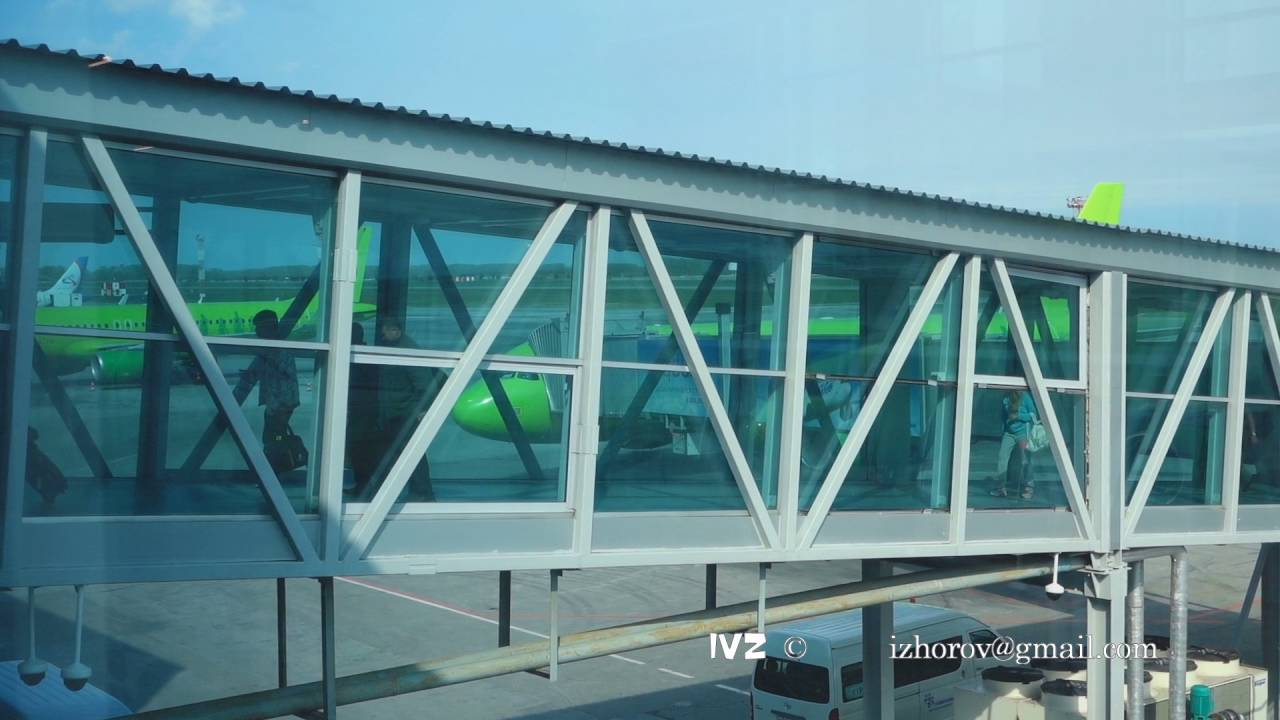
\includegraphics[width=13cm]{./images/Facade/access}
\caption{Access bridge connecting terminal and jetway.}
\end{figure}
	
	For the main bridge structure, steel alloys will be used for ceiling and floor, square shaped profile for vertical bars. Also, transversal beams of cylindrical profile will be used for tangential efforts absorption. 
	
	Asthetical finishings will be done keeping the facade aesthetics followed in the whole terminal building, for that reason the glass will use the same Spider system as presented before in section 5.1.
	
		\subsection{Emergency doors}
	Emergency doors have been subcontracted to the DORMA company. This company offers products for emergencies and escape route systems. 
	
	It has been chosen to use DORMA TV100 doors that are provided with locking devices that immediately unlock secured escape route doors on activation of the emergency pushbutton, in the event of an emergency and for authorized users. 
	
	They are equipped with an electromechanical locking mechanism and provide jam-free unlocking irrespective of loads. Doors are provided with an anti-corrosion protection, since they are made of a very sturdy metal. Furthermore, this system complies with the German guidelines on electrical locking systems for doors used in emergency exits and escape routes (EItVTR).
	
		\begin{figure}[ht!]
	\centering
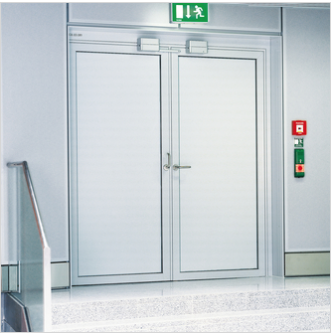
\includegraphics[width=9cm]{./images/Facade/emergencydoor}
\caption{Emergency doors provided by DORMA.}
\end{figure}
		\subsection{Automatic baggage handling system doors}
	ABHS (SATE) access from apron and vice versa, has been decided to be made with a series of doors distributed by all around the building, with the purpose of promoting the efficiency and quickness in loading and unloading baggage. These doors would be roll-up doors, since this way, the door can remain open without disturbing the operators, and be closed when activity is finished. As a consequence, the indoor temperature and humidity can be kept; therefore, reducing heating consumption inside of the building.
	
	The doors chosen have been from the company Stormtite, and the model is AP Model 627. These doors answer the demand for reliability, durability, flexibility and thermal efficiency. 
	
			\begin{figure}[ht!]
	\centering
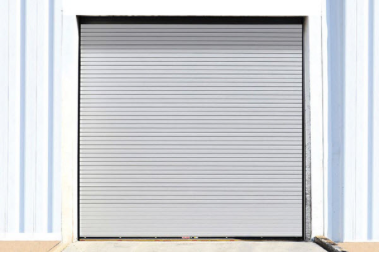
\includegraphics[width=9cm]{./images/Facade/sate}
\caption{Stormtite AP Model 627 doors for ABHS (SATE).}
\end{figure}
	
	

\chapter{Building cover}
	
	\section{Adopted solution}
	
	\section{Shape and inclination of the building cover}
		
	\section{Used materials}
		
	\section{Sewer system}
\chapter{Indoor closures}
	
	\section{Walls}
	
	\section{Doors}
		\subsection{Baggage claim hall doors}
		\subsection{Office access and automatic baggage handling system access doors}
		

\chapter{Fire prevention}
% COMMENT
\paragraph{} Airport Category nº9:  discharge rate of foam solution/min and water according to foam meeting performance level A.

Fire-Fighters station with two floors linked with vertical slide bars and stairs. 

\begin{description}
	\item[Ground level:] a quick and direct garage for 3 vehicles, plus lockers and depot.
	\item[First floor] with all the facilities such as gym, rest area, bedrooms, washroom, dinning room and infirmary.
\end{description}
% END COMMENT
Central location to guarantee a quick performance.
EXTRA:  Jakarta Fire Extinguisher at 25 km approx.

	\section{Fire prevention regulations }
		\subsection{Level of protection}
		\paragraph{} From ICAO Annex 14 V1, the level of protection at an aerodrome for rescue and firefighting should be equal to aerodrome category determined using the principles in articles \textit{9.2.5} and \textit{9.2.6}.
		
		Table \ref{table91} is used to determine the aerodrome category taking into account the longest aeroplanes normally using the aerodrome.
		
		The biggest plane using the aerodrome is the Boeing 777-300 which have a length of 74m and a fuselage width of 6.2m.
		
		According to this data, the \textbf{Aerodrome category} is \textbf{9}.
		
		\begin{figure}[H]
			\centering
			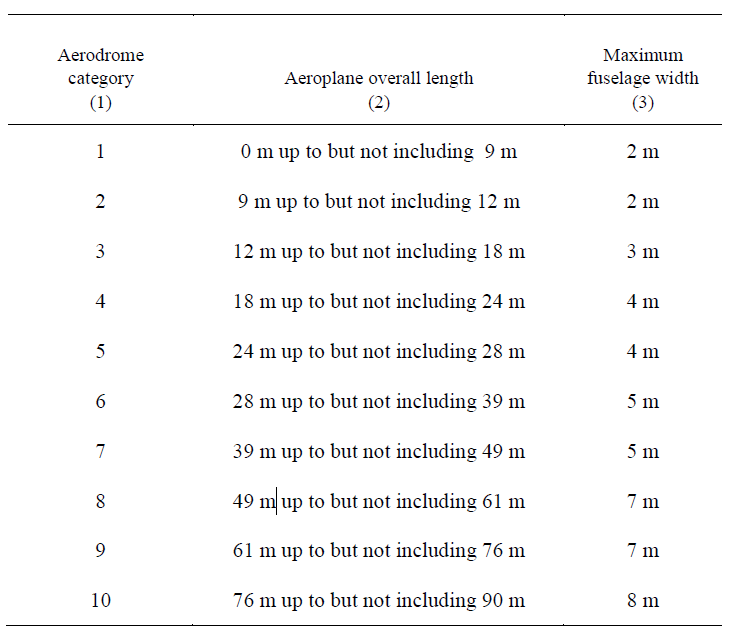
\includegraphics[clip, trim=0cm 0cm 0cm 0cm, width=0.8\textwidth]{./images/firefighting/table91}
			\caption{Aerodrome category for rescue and firefighting.}
			\label{table91}
		\end{figure}
	
		\subsection{Extinguishing agents}
		\paragraph{} Also, from ICAO Annex 14 V1, section 9, the amounts of water for foam production and the complementary agents to be provided on the rescue and firefighting vehicles shall be in accordance with the aerodrome category.
		
		From \textit{Airport Services Manual (Doc 9137), Part 1} and the category of the airport, the level of performance selected is \textbf{level A}. Now the table \ref{table92} can be used to determine the minimum usable amount of extinguishing agents for the airport.  
		\begin{figure}[H]
			\centering
			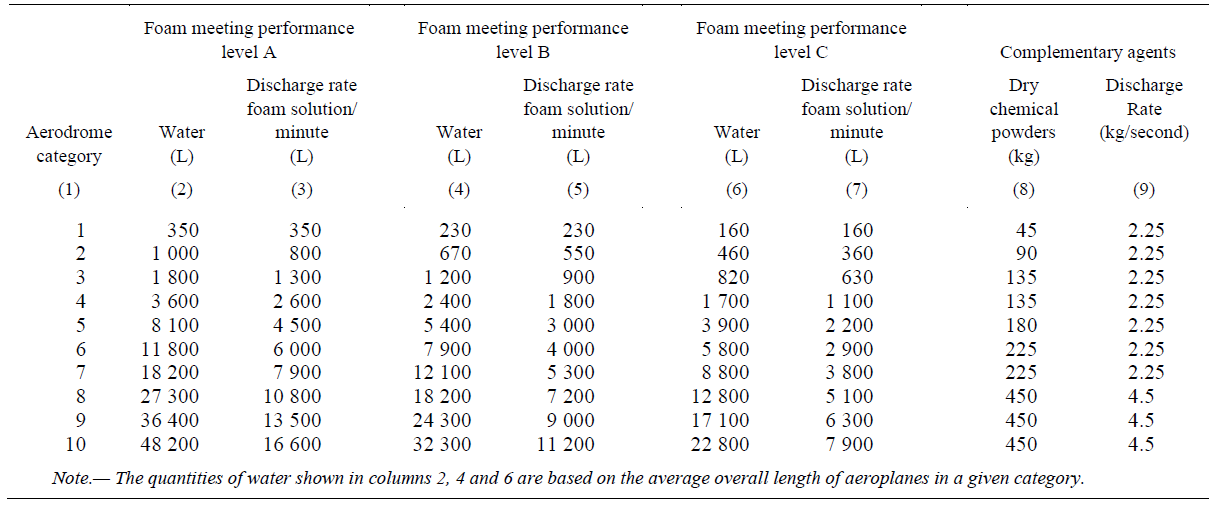
\includegraphics[clip, trim=0cm 0cm 0cm 0cm, width=1\textwidth]{./images/firefighting/table92}
			\caption{Minimum usable amount of extinguishing agents.}
			\label{table92}
		\end{figure}
	
	For a category 9 aerodrome with performance level A, the minimum usable amount of water is 36400 L and 13500 discharge rate foam solution per minute, for 450kg of dry chemical powders with a discharge rate of 4.5kg/s.

	Following the directives from article 9, the amount of foam concentrate provided on a vehicle should be sufficient to produce at least two loads of foam solution. Foam concentrate carried on fire vehicles in excess of the quantity identified in Table \ref{table92} can contribute to the reserve.
\section{Chosen materials}
		\subsection{Building elements}
		\subsection{Materials}



% BIBLIOGRAPHY

% styles:
%	abbrv   : [#] Initial. Surname (pages and vol. abbrev.)
% 	acm     : [#] Surname, Initial. (sc)
%	alpha   : [Abrev.yy] Name Surname
%	apalike : [Surname, yyyy] Surname, Initial 
%	ieeetr  : [#] Initial. Surname (pages and vol. ext.)
%	plain   : [#] Name Surname
%	siam    : [#] Initial. Surname (sc)
%	unsrt   : [#] Name Surname

\nocite{*}
\bibliographystyle{IEEEtran}
\bibliography{IEEEabrv,PROYECTO_AEROPUERTOS} 

\end{document}